\documentclass[12pt,a4paper]{article}

% German language support
\usepackage[utf8]{inputenc}
\usepackage[T1]{fontenc}

% Additional packages
\usepackage{amsmath}
\usepackage{graphicx}
\usepackage{hyperref}
\usepackage{geometry}
\usepackage[table]{xcolor}
\usepackage{fancyhdr}
\usepackage[backend=biber]{biblatex}
\addbibresource{main.bib}

\graphicspath{ {./figures/} }

% Page layout
\geometry{margin=2.5cm}
\pagestyle{fancy}
\fancyhf{}
\fancyhead[L]{SemanticWebBrowser}
\fancyhead[R]{\today}
\fancyfoot[C]{\thepage}

% Document information
\title{From Pocket-Inferer to SemanticWebBrowser:\\Architectural description of a user-friendly, deterministic, language-interface-based, web-paradigm-agnostic, IDE-like, energy-efficient Web-Browser}
\author{Jan Bingemann}
\date{\today}

\begin{document}

\maketitle

\newpage
\tableofcontents
\newpage

\subsection*{Abstract}

Why do official clerks not have the equivalent of a calculator like engineers do but for inference?
The fundamental idea of this paper is for ChatGPT-like apps to lose natural language for less energy consumption and more determinism in their answers based on controlled natural languages like ACE; and to capture this new paradigm in a new type of browser that has natural language as its primary interface, here called a semantic web-first browser.
The idea is proposed in several design steps, beginning with a simple to use calculator-like program to do inference with natural language, for which, when a programmer-mode is turned on, transforms into an IDE-like ACE-editor.
The idea is then further developed into a semantic web browser, which can also reference data and queries from the semantic web and later, it is philosphised how a web-paradigm agnostic SemanticWebBrowser could be realized.
This proposes a fundamental anthesis to ChatGPT-like apps and LLM-centered visions for the WWW with the biggest merit being to tradeoff natural language for more precision and less energy-consumption through controlled natural language.

%%The basic assumption of this paper is that the main reason why the semantic web has not had a break-through yet is, because its merits have not yet found its way to the end user, because there has not yet an interface been found to interact with the semantic web in a meaningful way that appeals to the masses.
%%However, because of their high energy consumption as well as their lack for precision, pure AI browsers do not seem to suitable for daily usage.
%%In this paper, controlled natural language is introduced as a main way to interact with the semantic web and based on this observation, the architecture for a semantic-first web browser is proposed.

The five main points this paper makes are:

\begin{enumerate}
    \item AI browsers with their high energy consumption are not suitable for daily usage (not in the near future, if ever).
    \item There has not yet been found a sufficient interface for the semantic web to be appealing to end-users and reach wider adoption
    \item Controlled natural language like ACE could serve well as a main interface for semantic data, because they manage to capture the potential of semantic web data better than any visualization ever could
    \item The best application for this approach would be a new kind of browser, which realizes ``language as an interface'' for the semantic web
    \item Derived from language as the main interface, the browser needs to center around the interaction with language and therefore look like a text editor or IDE.
    \item While showing the merits of the semantic web, the browser should also be ``backwards compatible'' with the traditional world wide web.
\end{enumerate}

It is largely based on the following work: \cite{semanticWebAce}.

\section{Introduction - A CLI for the WWW, or: finding an interface for a semantic web browser that is useable}

This text is a description of a next level SemanticWebBrowser, which tries to achieve various properties of semantic web applications in one app with a focus on semantic web data and technology. However, the problem here is that the current web is fragmented and there needs to be a mechanism to bridge the gap here. For this, controlled forward propagation is introduced as a potential solution:

The innovation here would be to combine Neuro Symbolic AI with ACE to achieve a language-based interface (controlled natural language as an interface), expand on the "Neural | Symbolic"-AI-approach with the controlled forward propagation mechanism to overcome the limitations of the mismatch between different web paradigms without losing the semantic-web-defining precision and determinism (paradigm agnostic but deterministic), as well as to stay to a reasonable degree energy-efficient, and to build a IDE-like semantic web browser from it all.

Its a combination of three main idea, which have all been explored before but not combined into one product:

\begin{itemize}
    \item A semantic web browser with an IDE-like, language-based interface to explore the semantic web (see:~\cite{semanticWebBrowser}, \cite{headlessBrowsers})
    \item Using ACE as a semantic web interface to increase usability over more formal query-languages and decrease energy-consumption over pure natural language (see: \cite{semanticWebLanguageBased}, \cite{semanticWebControlledEnglish}, \cite{semanticWebAce})
    \item Using LLMs to achieve web-paradigm agnostic semantic queries without losing determinism and semantic precision, and stay energy-efficient to a reasonable degree; both for input data and communication with external interfaces (see: \cite{llmAsDataTranslator}, \cite{llmForIntegratingHeterogenousData}, \cite{neuroSymbolicAi}, \cite{domainDiscoveryTool}, \cite{schemaInference})
\end{itemize}

The paper first describes the philosophical reasoning that lead to the idea.
Afterwards the four different implementation-stages of the SemanticWebBrowser are described.
The paper finishes with a conclusion.

\section{Paper-Overview and philosphical derivation for idea}

The semantic web has not yet had its ``iPhone''-Moment like AI with ChatGPT. This is because while having a database and backend just like regular WWW apps, semantic apps never figured out their frontend. That's the UI of a semantic web app? How does a browser for the semantic web look like?

I think the final puzzle piece that many people didn't make was that the semantic web would be controlled by a controlled language like Attempto Controlled English. With it, people could browse the semantic web, control agents, make order, etc.

A semantic web browser, therefore, would not be visuals-first (which, for our current state of mind is very contra-intuitive) but language-first (see language as an interface), a window into the world of semantic text. The semantic web browser feels therefore much more like a text editor or an IDE than a browser, which in the extension of apps, has become more and more like television, the semantic web browser will feel again much more like an interactive text document.

With the semantic web browser, society can make the next step from information society (informationsgesellschaft) to knowledge society (wissensgesellschaft), and maybe, someday, even let the digital behind us for good by controlling the material world through language.

\subsection{What is a semantic web browser? Or: the four different development stages}

There are basically three main stages:

\begin{enumerate}
    \item PocketInferer: Program for logical inference based on ACE
    \item AceCode: AceCode editor with the possibility to upload from simple external data sources like a CSV or SQL file but no semantic web integration
    \item SemanticWebBrowser: Possibility to also reference semantic web data
    \item Web-Paradigm-Agnosticism SemanticWebBrowser: Possibility to reference sources from different web paradigms (social web, agentic, traditional web)
\end{enumerate}

An overview can be seen in the following table:

\begin{table}[h]
    \centering
    \begin{tabular}{|l|p{2.5cm}|p{2.5cm}|p{2.5cm}|p{2.5cm}|}
    \hline
     & Energy-Efficient, Deterministic & IDE-Like, Language-Interface-based & Web-Paradigm-Agnostic & SemanticWeb-Support \\
     \hline
    Vibe Coding Tool & \cellcolor{red!25} No & \cellcolor{green} Yes & \cellcolor{red!25} No & \cellcolor{red!25} No \\
     \hline
    AI Browser & \cellcolor{red!25} No & \cellcolor{yellow} Semi-Yes & \cellcolor{green} Yes (based on ML) & \cellcolor{yellow} Semi-Yes \\
    \hline
    Social Media Client & \cellcolor{green} Yes & \cellcolor{yellow} Semi-Yes (Bots) & \cellcolor{yellow} Semi-Yes (Bots) & \cellcolor{yellow} Semi-Yes (Bots) \\
    \hline
    Traditional Browser & \cellcolor{gray!25} Depends & \cellcolor{gray!25} Depends & \cellcolor{green} Yes & \cellcolor{yellow} Semi-Yes \\
    \hline
    Ontology Editor & \cellcolor{green} Yes & \cellcolor{red!25} No & \cellcolor{red!25} No & \cellcolor{green} Yes \\
    \hline
    IDEs & \cellcolor{green} Yes & \cellcolor{green} Yes & \cellcolor{red!25} No & \cellcolor{red!25} No \\
    \hline
    Pocket-Inferer & \cellcolor{green} Yes & \cellcolor{yellow} Semi-Yes & \cellcolor{red!25} No & \cellcolor{red!25} No \\
    \hline
    AceCode & \cellcolor{green} Yes & \cellcolor{green} Yes & \cellcolor{yellow} Semi-Yes & \cellcolor{red!25} No \\
    \hline
    SemanticWebBrowser (SWB) & \cellcolor{green} Yes & \cellcolor{green} Yes & \cellcolor{yellow}Semi-Yes & \cellcolor{green}Yes \\
    \hline
    Web-Paradigm-Agnostic SWB & \cellcolor{yellow} Semi-Yes & \cellcolor{green}Yes & \cellcolor{green}Yes (based on ML) & \cellcolor{green}Yes \\
    \hline
    \end{tabular}
    \caption{Feature comparison table of browsers from different web paradigms}
    \label{tab:features}
\end{table}

\subsection{Terms}

The paper differentiates four main web paradigms:

\begin{figure}[h]
    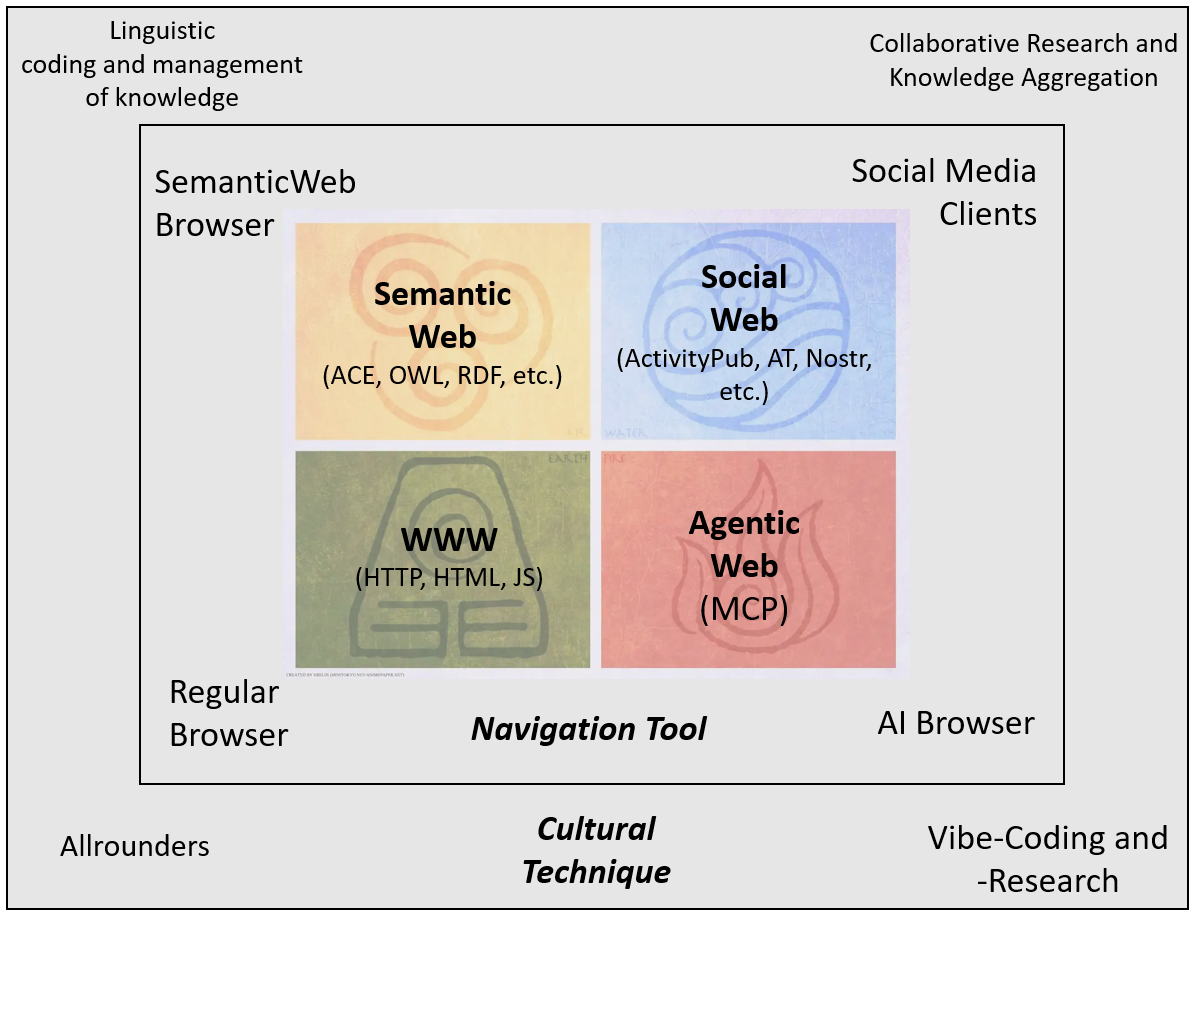
\includegraphics[width=16cm]{different_web_paradigm}
\end{figure}

The term social web also includes all commercial social media platforms like Threads or X, which by now also feature bots with which one can interact with and in a way, browse other web paradigms.
The same is true for apps like ChatGPT, which in a way, allows to browse the traditional web, semantic and social web, because it either used much of this data for training, or, because it actually gets data on demand.

TODO: Do some research if there are some references

\subsection{What would be the benefit of a semantic web browser (and a semantic web) in public administration of finance?}

People could reference and query data, send mails, etc.

\subsection{What is the role of LLMs here?}

Agents on the web can be programmed much more deterministically than through LLMs. Of course, LLMs can help generated ACE code. Vibe coding exists here just as on the regular WWW.

\subsection{Why is it necessary?}

Why do we need a semantic web browser? Currently, we see that more and more people speak like LLMs, which means that the text that LLMs train upon, looks more and more similar. At the same time, companies are spending more and more energy on the training of LLMs to make the same language even more powerful. This means a impoverishment of language while at the same time the same semantics are tried to be made more powerful (in a very literal sense) with every more energy.

In practical terms, a language-driven semantic web browser would flip many ways that we interact with the web today. Instead of navigating digital spaces with a certain goal in mind, the user would instead formulate what they want in a pre-defined language and then have the web execute the rest. This means, that user is closer again to achieving what they want from browsing, which they often know beforehand, instead of being confronted with a UI in which they somehow need to figure out how to achieve a goal that they already know. Of course, formulating a goal comes with its own challenges, but here, templates that could be shared between users could be of use here, and potentially, also LLMs.

\subsection{What about traditional WWW?}

Rather than ``semantic web browser'' it should be called ``semantic-first web browser''. The semantic web is an extension of the traditional web, but it could be useful to flip which data is interacted with primarily, because central design choices depend on this: since the best way to interact with the WWW is visually, WWW browsers focus on visuals while the semantic web is best navigated with language, a semantic-first browser should focus on language.

However, while already in browsers, it is possible to interact with semantic web data, it should of course still be possible in semantic-first browsers to interact with traditional web data. And possibly for a very long time (or maybe always for web browsers), this will be necessary, for example if a web service only provides a REST API.

For example, let's consider the users wants to buy new running shoes on Amazon. They could enter a text which references the ontology of Amazon. However, since Amazon requires a sign in, the user would be directed to a sign-in page. After signing in, the prompt's execution would continue, and the credentials would be saved in the semantic browser possibly for later.

In other occasions, the content is just better visualized, so there should be the possibility for websites to still render replies in html.

Problems would quickly arise from interacting with data that is only provided via a REST API. The only solution I can think of here would be either to let the user manually map objects to the current ontology, which would be tedious, or that an LLM would do the same, which would be unreliable.

Generally, of course, it would be the best if more and more web services would also provide a semantic web interface for semantic browsers to interact with them.

\subsection{How would the UI look like?}

Since language is the primary interface, it would look like a text editor or an IDE. Also, it should be possible to reach web services and ontologies from the WWW through import-like statements in ACE.

\subsection{What's the cultural impact?}

In many ways, the semantic browser would stand against the AI-driven browser. And while the AI-driven browser is of course much more user-friendly, the semantic-first web browser would be much more energy efficient, more deterministic and would keep the emancipating aspect of language intact.

Additionally, it stands in contrast to vibe-coding:

\begin{enumerate}
    \item Instead of ``everything goes'' the parser excepts a given syntax. Therefore, users need to be precise instead of improving the output with blurry prompt-engineer ``rules''.
    \item It's not expected to have the prompt ready right from the start. Users are invited to spend time crafting and polishing their ``prompts'', before they execute them.
    \item The prompts are treated more like one whole source code that is optimized over time rather than a history of chat exchanges, which is re-created on every new prompt. Therefore, the UI looks more like an IDE than a chat. The user is creating code that stabilizes incrementally over time rather than having changing/deleting/removing parts of the code by the AI at random, hoping that parts of the code will eventually stabilize because of a lucky prompt.
\end{enumerate}

The fundamental idea behind all of this is to give users back control on their language, with which they interact with their data as well as the underlying description of whatever they are trying to create/describe or retrieve. Instead of the alchemistic streak that vibe coding has, ACE-coding emphasizes the ``engineering''-aspect of ``prompt-engineering''.

One can observe that the semantic-first browser blurs the line between browsing and coding. In a way, the semantic-first browser integrates the browser's development tools into the browser-experience. Instead of having a rich UI and a small search bar/console, the browser becomes a rich search bar/console with a small visual component. The idea feels similar to how the console and bash scripts are used on Unix systems -- as a power user tool but for the web instead of operating systems.

Through this, of course, the initial threshold becomes much higher. But maybe, these are cultural techniques that need to be educated in a modern knowledge society. Maybe it's fine that certain skills are necessary to interact with technology and that's it not merely about a strong will to do whatever it takes, but requires the aggregation of knowledge, learning of skills and cooperation between individuals. And language is and has always been an important tool here.

\section{Pocket-Inferer (potential Predecessor, german: Taschenfolgerer)}

As a potential predecessor, a simple ACE-based logical inferer could be implemeted, which when enabling a Programming-Mode, changes to AceCode.

\begin{figure}[h]
    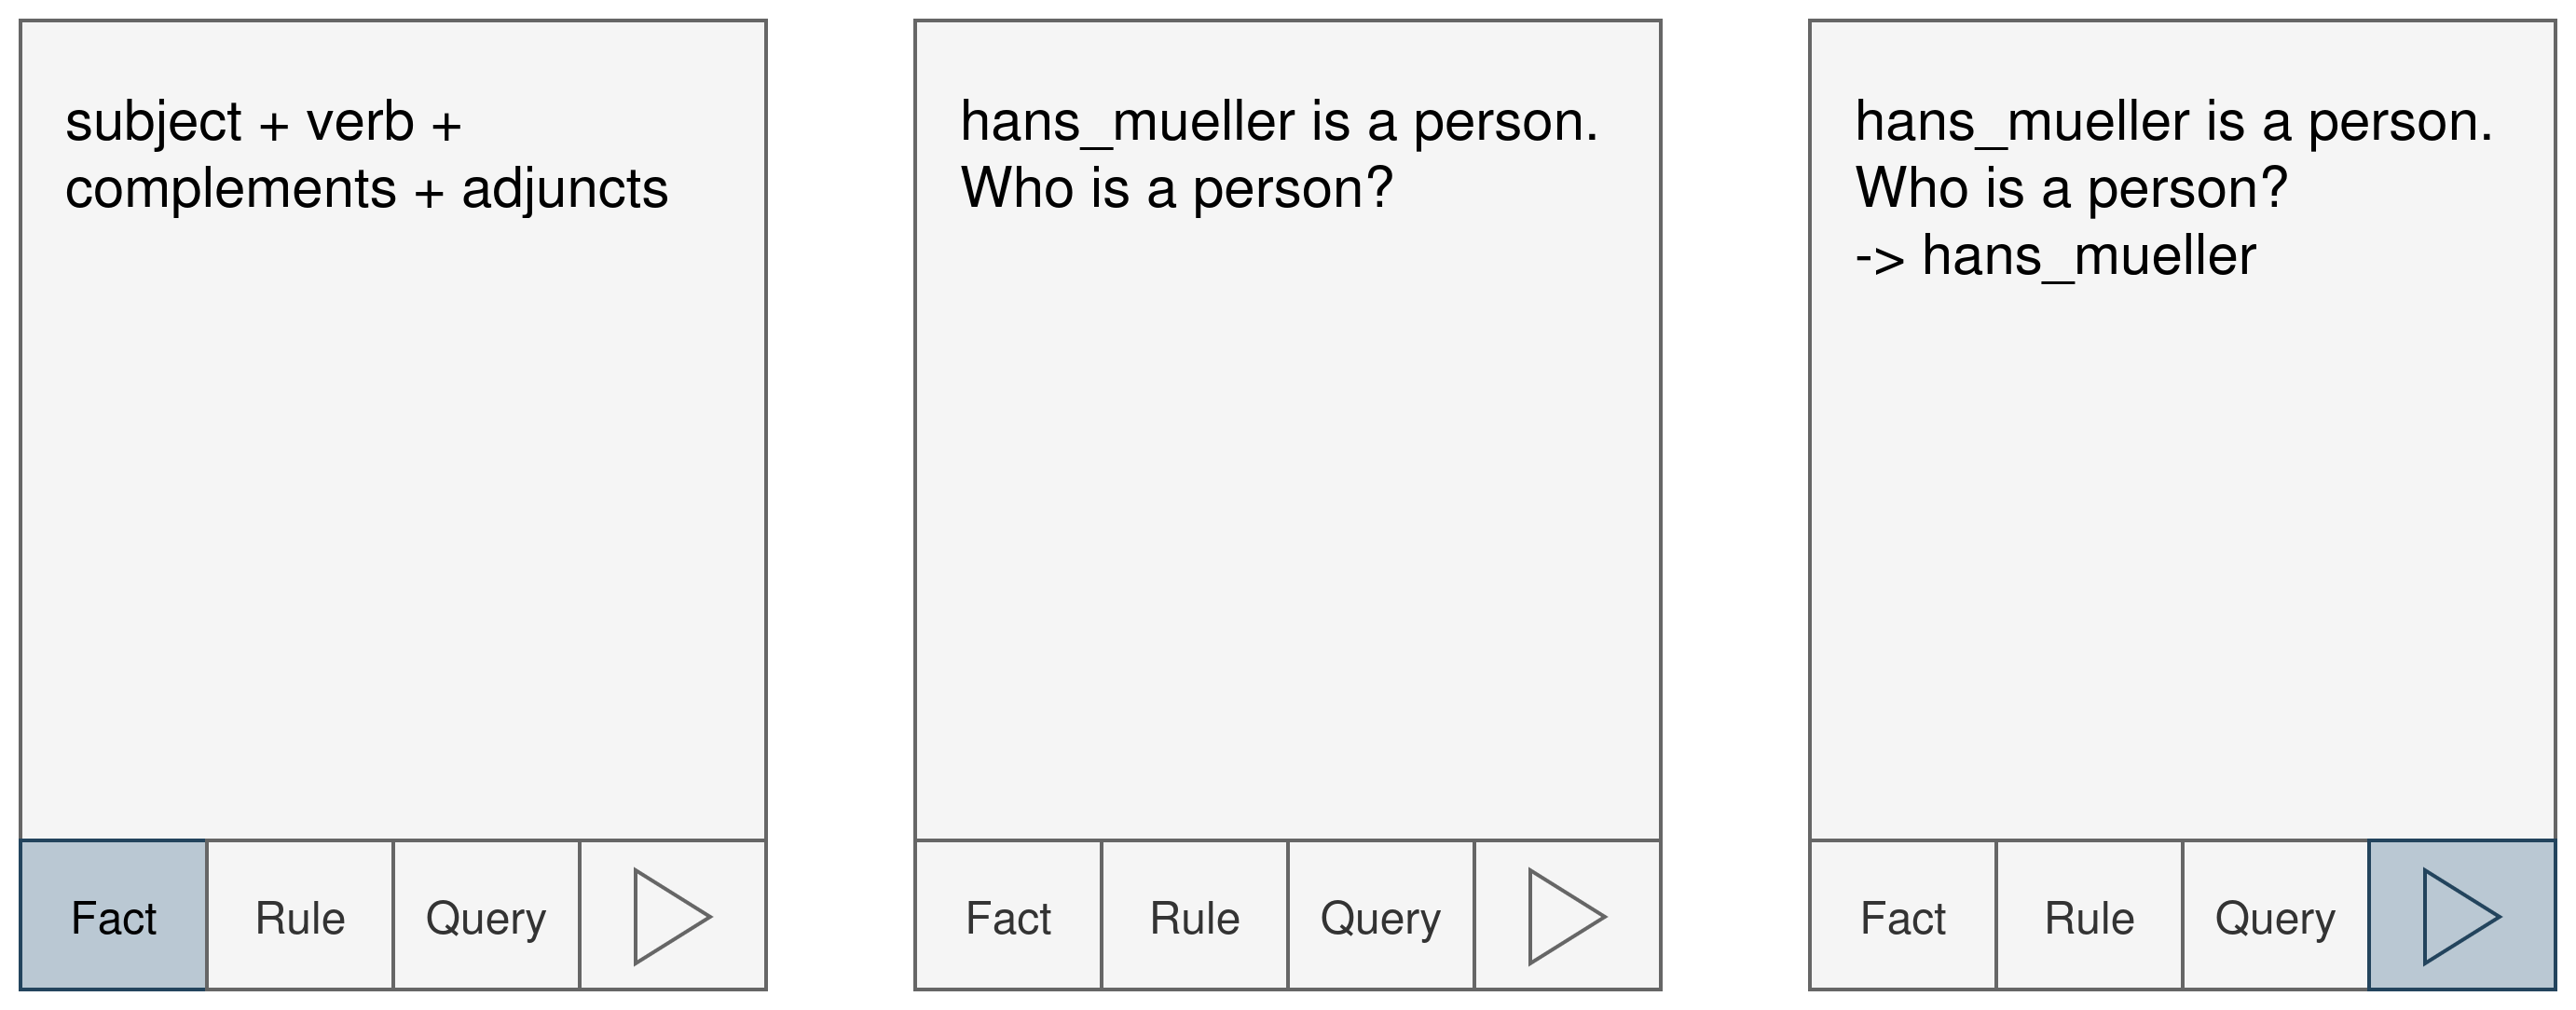
\includegraphics[width=16cm]{taschenfolgerer}
    \caption{Pocket-Inferer (Taschenfolgerer)}
\end{figure}

\section{AceCode (IDE for logical inference based on ACE)}

The following sections describe the next step: an IDE for logical reference based on ACE.

\subsection{Behaviour and Architecture}

And a visual representation of the behaviour of AceCode can be seen in the following figure:

\begin{figure}[h]
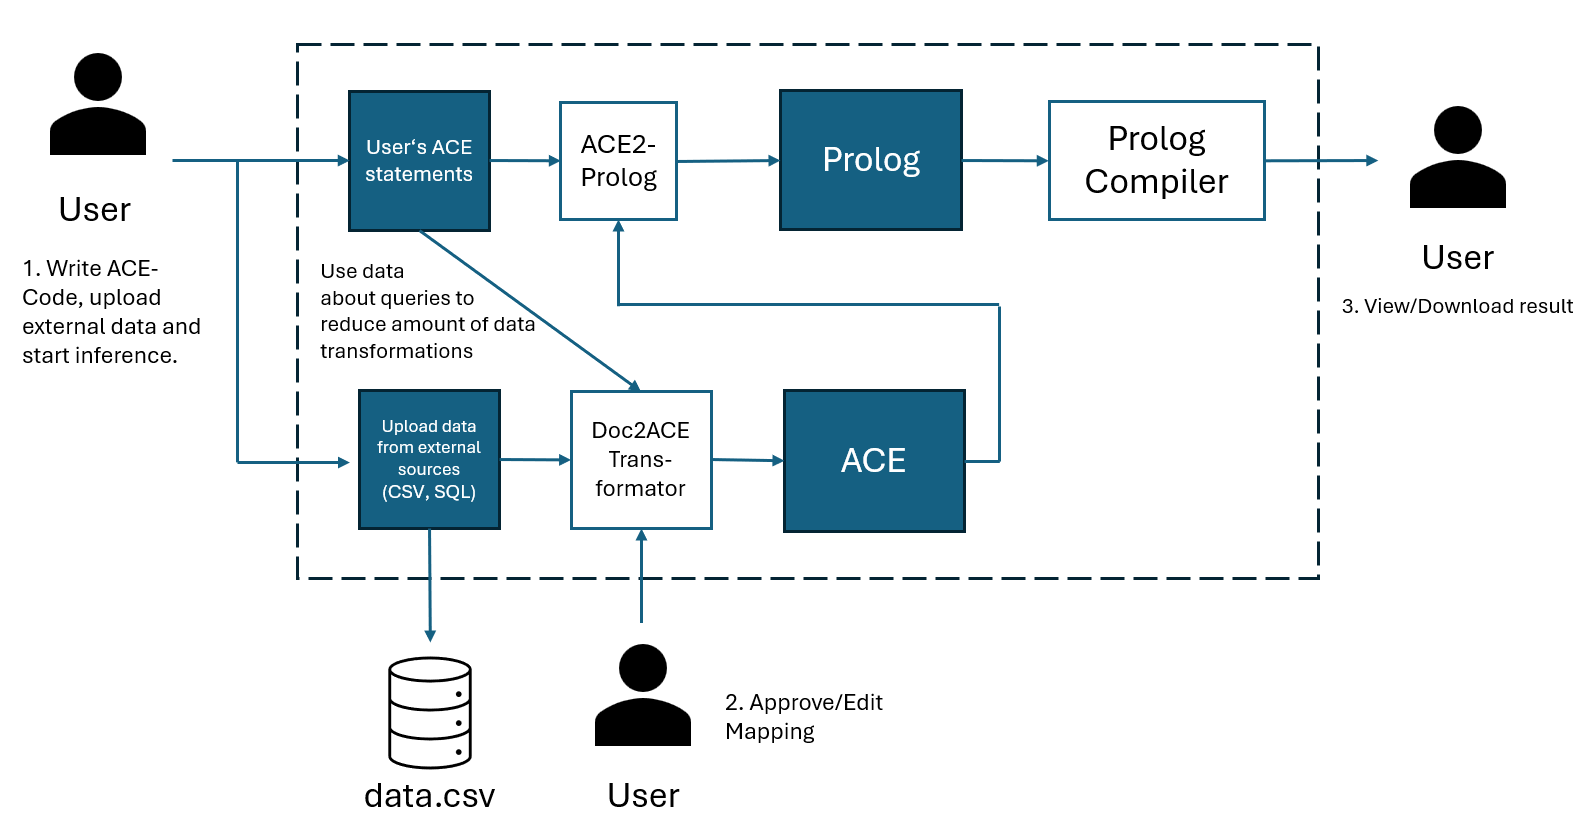
\includegraphics[width=16cm]{ace_code_state_diagram}
\caption{AceCode State Diagram}
\end{figure}

The idea is that, when the user wants to upload data from an external data source, to reduce the amount of data that needs to be turned into ACE, data conversion happens depending on the user queries (see~\cite{schemaInference}).

TODO: add diagram for architecture

TODO: Think about whether this should be a client or kubernetes application (write about both cases)

TODO: Think about integration with semantic web - is reference of semantic data enough?

TODO: Think about OWL - Is ACE an alternative, could it become the lingua franca of the semantic web? - Actually OWL can be used to define semantics. User should be able to load external OWL semantics as ACE code

TODO: Think about the current neuro-symbolic approach with turning everything into ACE is the most effective one (write about all other cases, too)

\subsection{User-Interface}

The user interface could look like the following:

\begin{figure}[h]
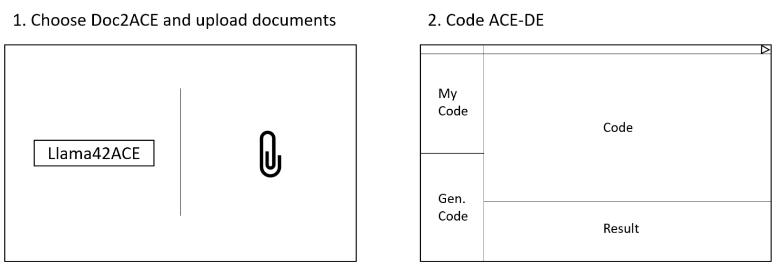
\includegraphics[width=16cm]{ui_mock}
\caption{AceCode User Interface}
\end{figure}

\subsection{Implementation of AceCode}

A first implementation of the first stage of the SemanticWebBrowser can be seen in the following figures:

\begin{figure}[h]
    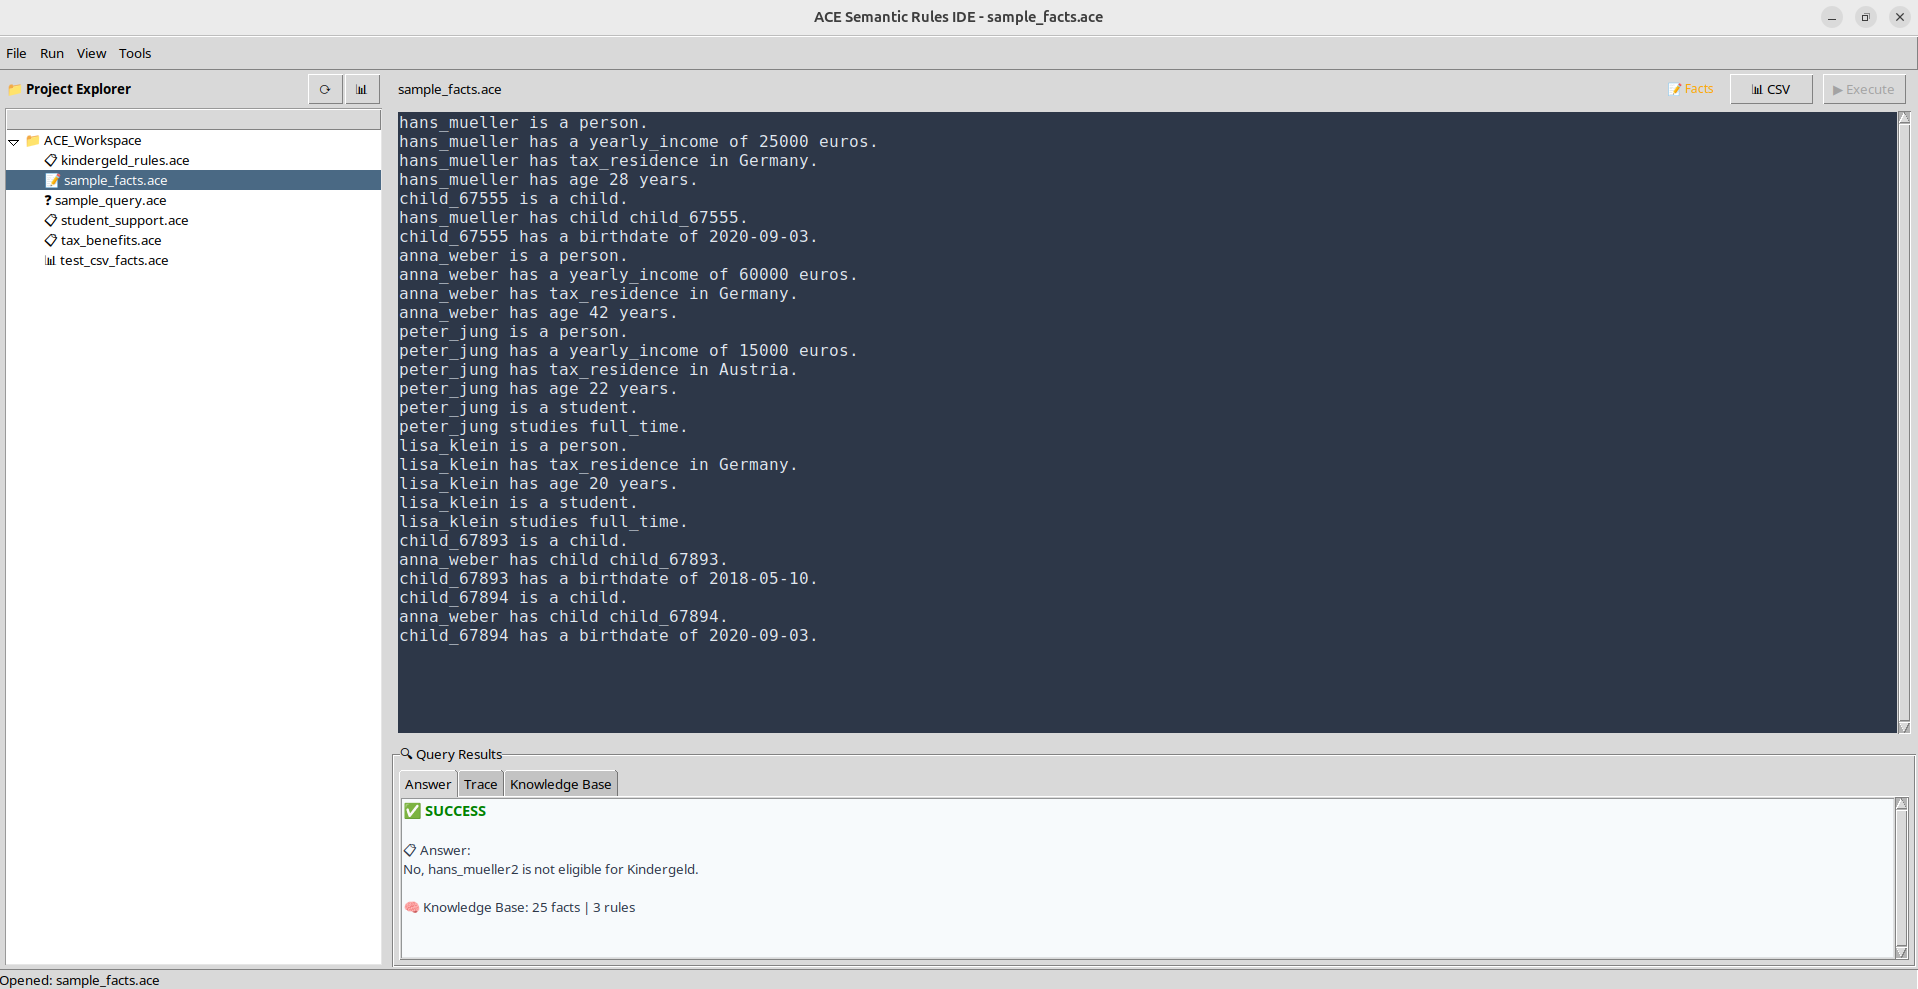
\includegraphics[width=16cm]{ace_code_screenshot_1}
\end{figure}

\begin{figure}[h]
    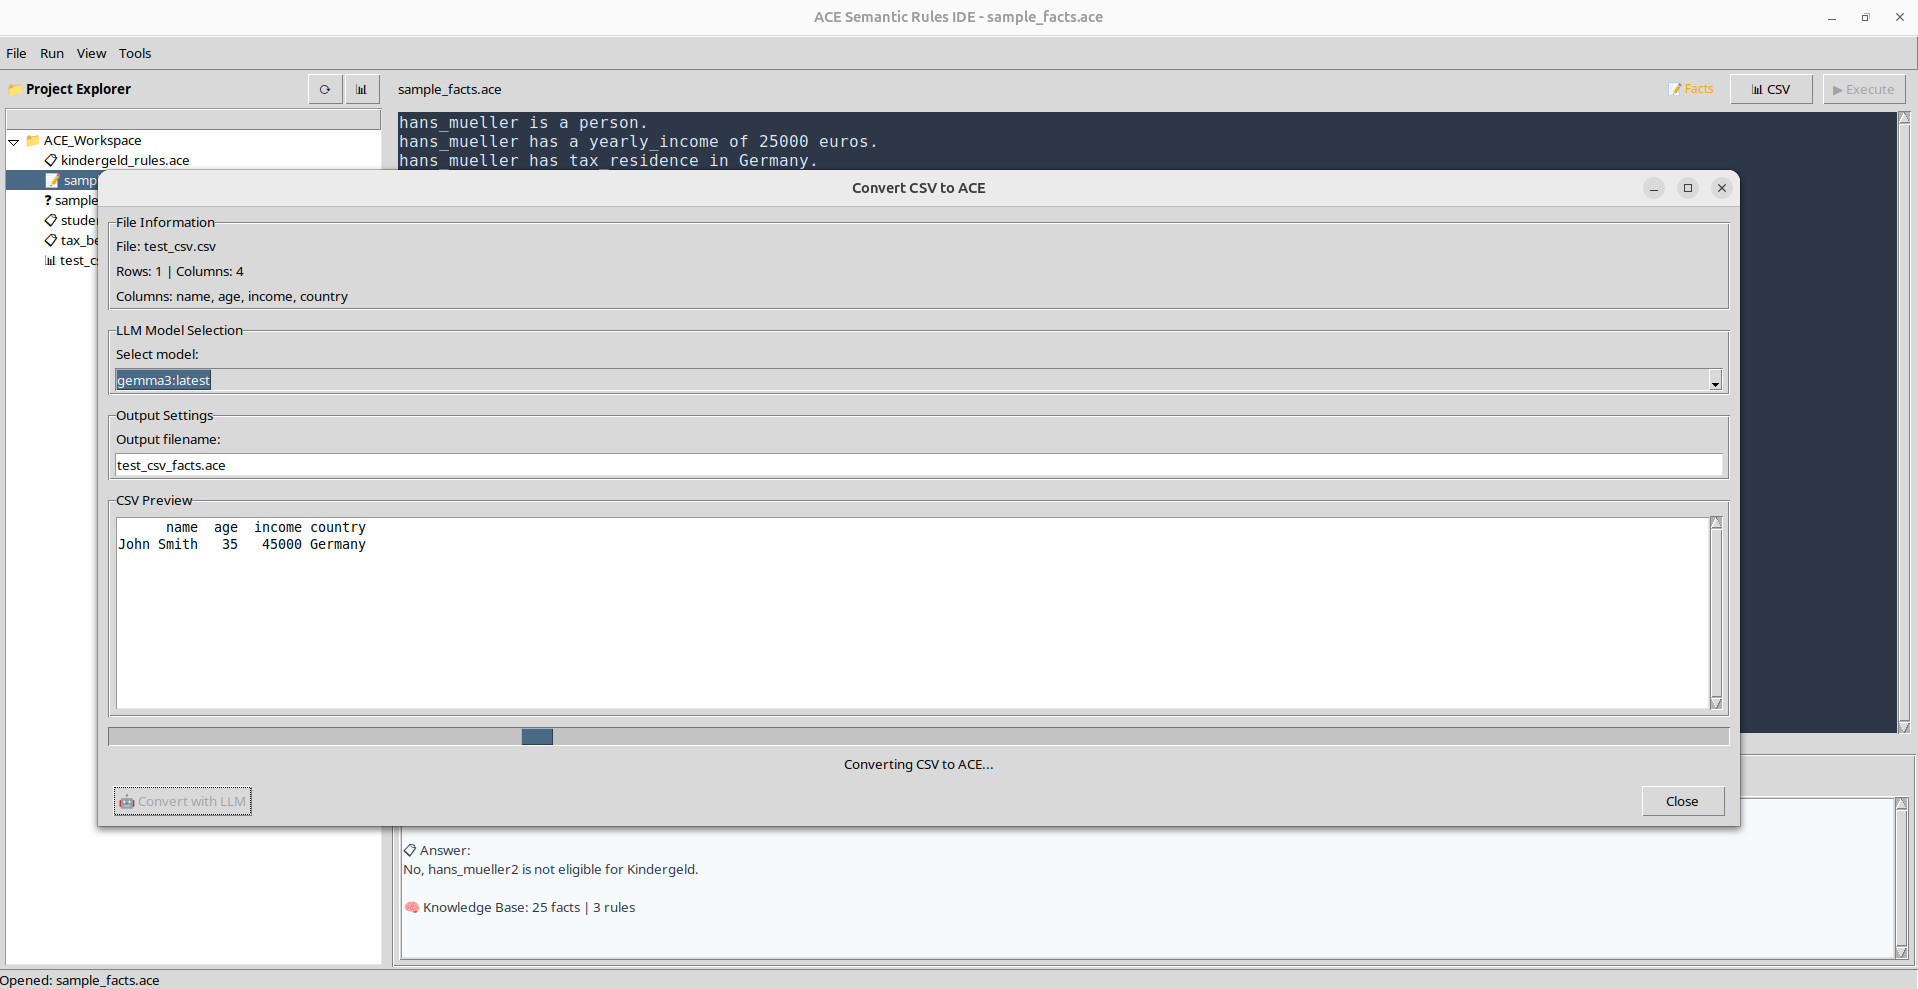
\includegraphics[width=16cm]{ace_code_screenshot_2}
\end{figure}

\begin{figure}[h]
    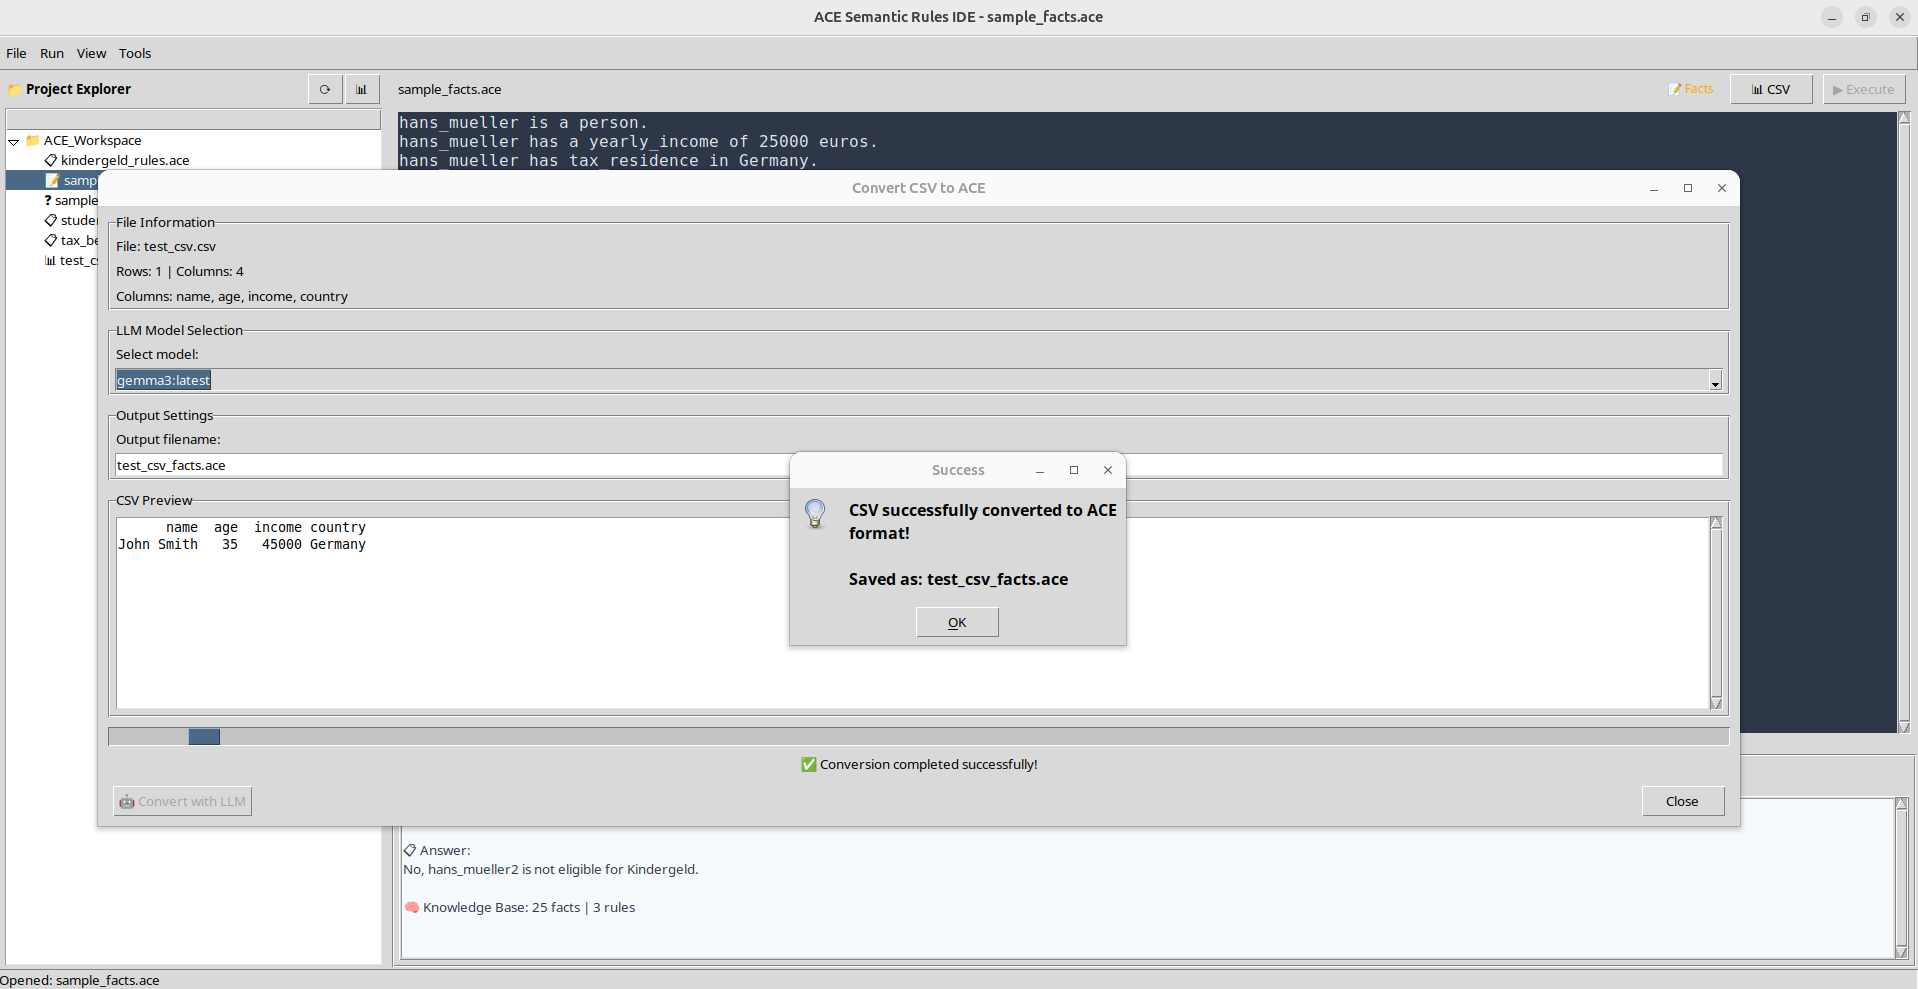
\includegraphics[width=16cm]{ace_code_screenshot_3}
\end{figure}

\begin{figure}[h]
    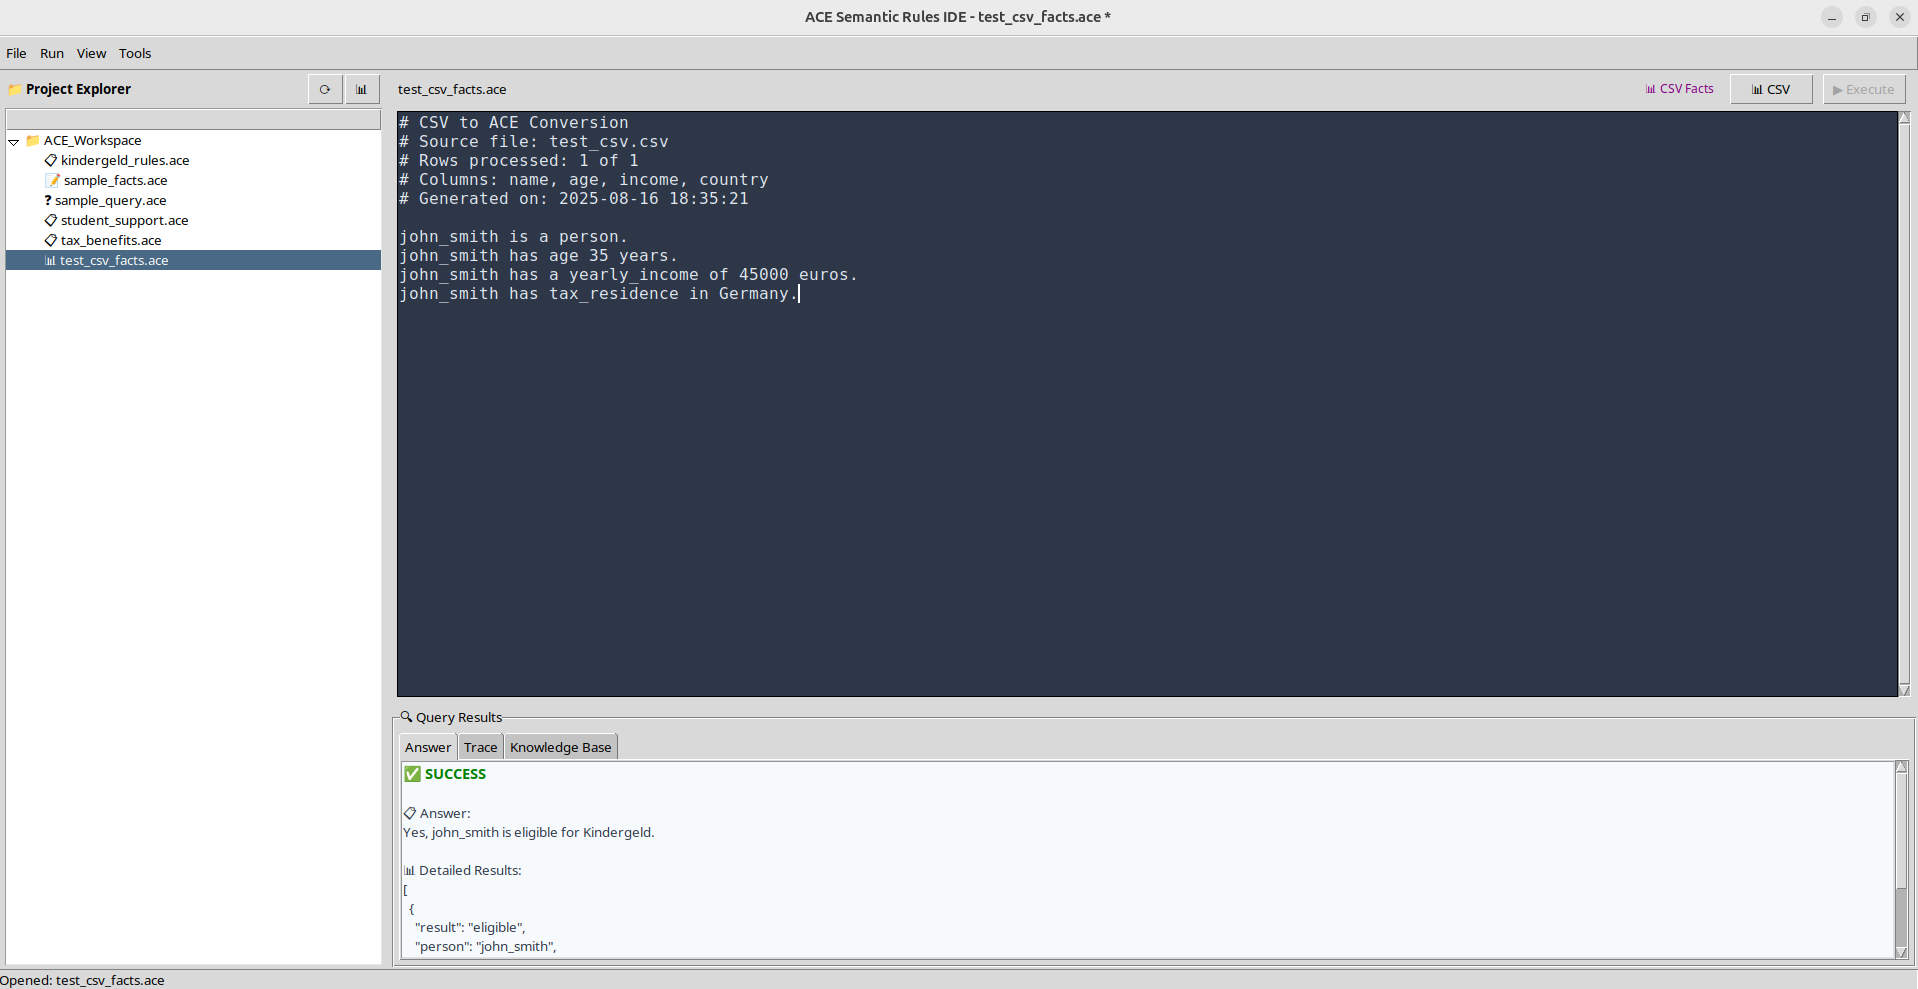
\includegraphics[width=16cm]{ace_code_screenshot_4}
\end{figure}

\section{SemanticWebBrowser Implementation from AceCode}

In the following section, the integration of the semantic web into AceCode is described.

\subsection{How would it be technically realized?}

Similar to APE, the parser engine of ACE (attempto controlled English). ACE is converted into prolog and then executed and the result returned.

The tech stack would be traditional semantic web technology, but with controlled natural language as the logic language on top (see the following figure from \url{https://www.researchgate.net/figure/Semantic-Web-technology-stack_fig4_318562452}).

\begin{figure}[h]
    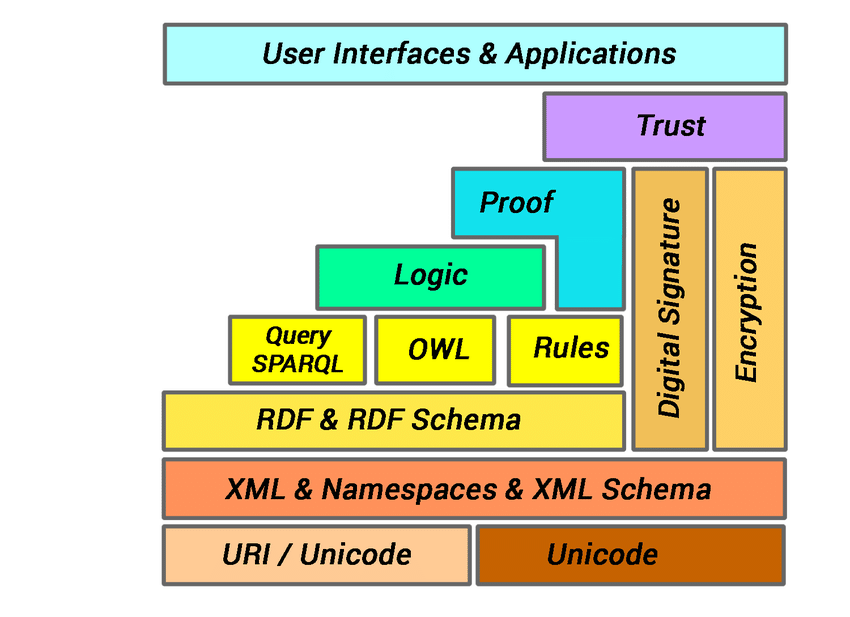
\includegraphics[width=12cm]{Semantic-Web-technology-stack}
    \caption{Semantic-Web technology stack}
\end{figure}

And try to introduce a new semantic web tech stack with a higher usability:

\begin{figure}[h]
    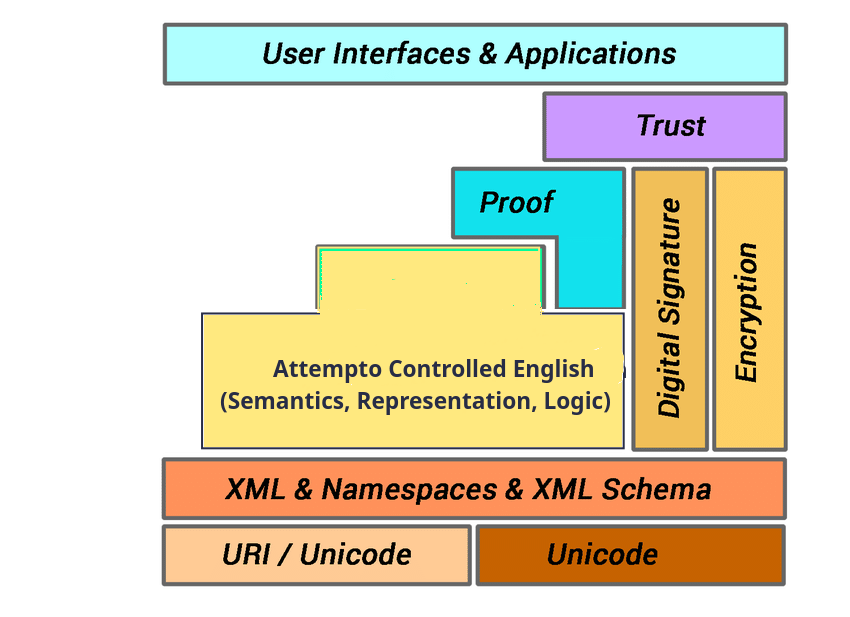
\includegraphics[width=12cm]{Semantic-Web-technology-ace-stack}
    \caption{Semantic-Web Ace technology stack}
\end{figure}

\subsection{Does it make LLMs completely obsolete? Introducing the precision controller.}

Is the semantic web browser a complete counterproposal to ChatGPT and LLMs in general -- no. The idea is that LLMs could be used to translate between different web paradigms (semantic-, AI- and REST-based), because pattern-recognition is what LLMs can do best.

Using a latch, users could specify how ``sharp'' the rules of the user's ontology are being propagated over the data that it finds on the semantic web. With a very low degree of ``sharpness'', the semantic web browser makes no use of LLMs and allows no deviation from the ontology and basically can only be used for semantic web data that fits the current ontology. With higher degrees, LLMs are used to access more data and access wider parts of the web, with the disadvantage of potential hallucinations, unexpected and wrong behaviour. Of course, this feature should be applied very carefully; however, if used sparingly, it could solve the current problem of mismatching ontologies and web paradigms that prevent a semantic web browser. In a way, a latch with a full degree of blurriness would actually simulate the MCP-protocol by Anthropic, in the sense that you have still the requirements by the controlled natural language, but the semantic web server would basically freely act, just like the MCP-Protocol does.

So, with the precision controller, the semantic web server actually can be turned into a ChatGPT from a different direction but also toned down again to a tool of sharp reasoning and precise and deterministic control of semantic web data.

One could also think about whether this precision controller could also be applied on the strictness that the ACE syntax is applied. With a higher degree of blurriness, even loosely formulated statements are accepted and then the ontology is also more loosely applied. This could also depend on how much energy the application should currently consume.

\subsection{AI Explainability}

Basically, with an app like ChatGPT, you have before you a black box that you can send commands to and that gives you unpredictable answers and consumes huge amounts of energy.

Instead, the semantc web browser with the precision controller starts with a complete white box, where you can control the ontology, have full control of the language, the outcome and consumes much less energy; but you can move on the ratio towards a ChatGPT-like black box with the precision controller.

With the default level, the ACE-syntax is enforced very strictly and semantic web data is expected to have the same syntax as defined. With a lower precision level, an LLM is stuck inbetween, syntax is not enforced as strictly and the ontology is enforced even if the data does not match it, also propagating to other web pradigms like MCP/AI-web and traditional web-services with REST-APIs.

The precision controller basically let's the user move between a very strict semantic web browser and the lose cannon of a ChatGPT+MCP-app. And I think this moving of ratio is only possible if you start developing a strict semantic web browser, which has a precision controller integrated.

Another merit is that the energy consumption can be adjusted at will. If money/energy is low, for example in a state's administration, the semantic web browser can still be used, while ChatGPT-like apps become unfeasible.

Everything else about the idea has already been implemented (e.g. see \url{https://www.cognitum.eu/semantics/fluenteditor/}); the new thing would be the precision controller, because LLMs haven't been around this long (and the real world is often not sufficient to model it with pure logical expressions) and combined with controlled natural languages like this. In an abstract sense, ChatGPT can already been thought of as a semantic web browser, as well as implementations like fluenteditor; however, while the former consumes too many resources (the hallucinations can probably be fixed), the later assumes a world that can be modelled with ontologies that does not exist and will always fall short of reality. The semantic web browser proposed in this paper could bridge this gap and create an application, that let's user browse the semantic web in a mature (``mündig'') way.

\newpage

\section{Web-Paradigm-Agnostic SemanticWebBrowser}

In the following section, domain discovery is tried to be implemented in a way to make the SemanticWebBrowser web-paradigm-agnostic.
The mechanism of domain discovery with the help of LLMs is in the following called Controlled-Forward-Propagation.
It was intended as a new mechanism for implementing a web-paradigm-agnostic semantic-web-browser, but is actually just domain discovery and an area of research for years.

Another approach is called wrapper generation (in the data mining context), which is used to scrape data from the web and turn it into relational form (first order logic).

\subsection{Introduction - What is Domain-Discovery?}

The current WWW is fragmented. Applications that allow the user to browse (or more broader speaking: explore) the semantic web fall short when it comes to overcoming the mismatch with other web paradigms (agentic/MCP web, social/ActivityPub/AT web or traditional WWW/REST web), as well as with data from other web paradigms like SQL. This paper introduces a novel mechanism to overcome this protocol/data mismatch by basically applying the user's ontology to new data/web interfaces using LLMs. LLMs are here not used for immediate translation of data/queries but are just used to generate the transformators, which are deterministic code, which is then used to transform the data. Therefore, it is also possible to check the generated transformator with the user and then use it to forward the request/process the data.

The innovation here would be to combine Neuro Symbolic AI with ACE to achieve a language-based interface (controlled natural language as an interface), expand on the ``Neural | Symbolic''-AI-approach with the controlled forward propagation mechanism to overcome the limitations of the mismatch between different web paradigms without losing the semantic-web-defining precision and determinism (paradigm agnostic but deterministic), and to build a IDE-like semantic web browser from it all.

\subsection{Principle}

In the following, domain discovery as well as different Schema-Mapping-Strategies based on LLMs are proposed to make the browser web-paradigm agnostic as well as compatible to other semantic ontologies.

The CFP-mechanism works by accepting a semantic web and facts as well as some sample data or interface specification, and returns a transformator-program, which can then be used to bridge the data/between the different web interfaces. It is depicted in the following figure:

The term Social Web here does not mean only mean decentralized social media networks based on ActivityPub and AT but also all centralized social media platforms.

\subsection{Implementation At the example of REST-based web-services}

CFP is used to bridge between semantic web representations like RDF (potentially displayed using controlled natural language like ACE) and other web paradigms using LLMs. It outputs a mapping in XML, which is then used by the transformator-program to apply the translation on the given data/query.

Because of the transparency of XML, the user is able to check the result of the LLM and accept/decline or make modifications to it. After this step, everything should be deterministic again. The LLM is only used for the generation of the mapping.

Of course, there could be different options for the user, which immediately accept everything the LLM generated without checking back with the user, however, this would come with the risk of hallucinations and therefore unexpected, false and even dangerous behaviour.

\subsection{CFP Example for a REST-based web service}

In the following, I want to demonstrate the principle with an example of a given RDF specification, an SPARQL-query and an OpenAPI-specification. CFP will be used to generate an XML-mapping, which is then fed into the transformator-program to translate the query and apply it to the REST-API and translate the result to RDF to display it to the user.

This example demonstrates the complete CFP workflow from user ontology to final query results.

Summary of CFP Process:
\begin{enumerate}
    \item LLM Input: User ontology + SPARQL query + OpenAPI spec
    \item LLM Output: XML mapping specification
    \item User Review: Validates/modifies XML mapping
    \item Fixed Engine: Processes XML mapping to:
    \begin{itemize}
        \item Translate SPARQL filters to REST parameters
        \item Execute REST API call
        \item Transform JSON response to RDF using mapping rules
        \item Execute original SPARQL on transformed RDF
    \end{itemize}
    \item Result: Semantic query results from REST data
\end{enumerate}

\newpage

\subsection{Moving the ratio between determinism and LLM-fuzziness}

Potentially, with different LLMs with different levels of fuzziness and energy-consumption, it would be possible for the user to be able to modify this trade-off-ratio at will based on LLMs (which is not possible when starting from a ChatGPT-like app).

\section{Conclusion -- A web interface, which can be adapted to the available resources and give back control to the user}

What about this paper is new? Basically, everything introduced here was already tried out before. However, the approach has not yet been implemented consequently in one product (that is a browser) and combined with LLMs in a productive way, as well as has been reduced in the past mainly to English:
\begin{itemize}
    \item Implementing ACE as an interface for the semantic web in a browser that has language as the primary interface has not been done before
    \item German as main language has received little research until now
    \item Using LLMs as translation-tools between AI/MCP web and traditional/REST web that can be applied to variating degrees (precision-controller) is new
\end{itemize}

The primary advantages of these approaches would be:
\begin{itemize}
    \item Lesser energy consumption than pure LLM approach
    \item Higher precision/determinism than LLM approach
    \item Could work against impoverishment of language: by separating ``social'' language from technical language, it could contribute to keeping the social aspects of language intact while giving people a better tool to collaborate in their technical endeavours.
    \item With the Precision-controller the advantages of ChatGPT-like applications can be applied when the risks are accepted, and the resources (money/energy) are available
    \item LLMs could offer a translation between different web-paradigms
\end{itemize}

In this sense, this paper introduces an implementation of a semantic web browser (with an interface based on natural controlled language and a precision controller based on LLMs) that flips the current approach to AI-based applications on its head by expecting a higher formality from the user input, but could contribute to a wider adoption of the semantic web, give more control back to the user and keep the emancipatory aspect of language intact. At the same time, the precision controller could enable a backwards compatibility with other web paradigms and keep the advantages of current ChatGPT-like applications if the user is willing to take the risks associated with this and is conscious about the energy-consumption of it.

CFP builds on existing approaches to bridge the gap between different web paradigms for implementing a protocol-agnostic semantic web browser. It could be used to implement a language-interface-based semantic web browser, with which user could have access to various data sources and query much of the web's data without relying solely on LLMs, which have a high-energy consumption and are unreliable and instead building on controlled natural language and using LLMs solely for the mapping between different web paradigms if necessary, and in such a manner that it can always be second-checked by the end-user.

\printbibliography

\end{document}
